
\chapter{Main Detector Monopole and Dipole Responses} 
\captionsetup{justification=justified,singlelinecheck=false}

\label{AppendixD} 

\lhead{Appendix D. \emph{Detector Dipole and Monopole}} 

\begin{figure}[ht]
\centering
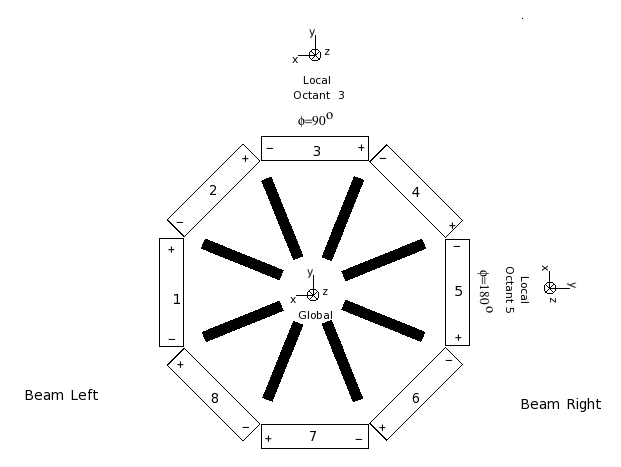
\includegraphics[width=0.7\textwidth]{Pictures/octant_coordinates.png}
\caption{Diagram of \Qs detector system looking downstream showing octant labeling. Numbered rectangles represent detector bars while solid spokes represent spectrometer coils.}
\label{fig:octant_coords_D}
\end{figure}
Consider the azimuthal arrangement of the main detector bars in Figure \ref{fig:octant_coords_D}. Response patterns on the azimuth, that is, responses as a function of main detector bar azimuthal location can offer clues as to the source or origin of the signal creating the response. For example, the response of the main detector to position or angle modulation as a function of the octant angle around the azimuth should have an approximately sinusoidal pattern. These sinusoidal patterns are referred to as ``dipoles'' and in the jargon of \Qs when the maximum response is in the vertical direction (maximum response on bars 3 and 7) it is referred to  as a ``vertical dipole''. Likewise when the maximum response is in the horizontal direction (maximum response on bars 1 and 5), it is called a ``horizontal dipole''. Thus, X-type modulations will create horizontal dipole responses and Y-type modulations are expected to produce vertical dipole responses. Any effect that creates equal responses in all detector bars is called a ``monopole response''. Shifts in energy and charge are candidates for monopole responses.

 Examples of dipole and monopole responses to the various types of X and Y modulation before and after correction using the full 10-Coil analysis can be seen in figures \ref{fig:Run2_10coil_Xdipoles} and \ref{fig:Run2_10coil_Ydipoles}. In these plots the dipoles are given as the amplitude of the sinusoid and the monopole as the center or offset of the sinusoid. A few observations can be made from the plots.

1. As expected, obvious horizontal and vertical dipole responses can be observed for X-type and Y-type modulations respectively. In both cases, these large dipoles are removed after correction suggesting that the modulation analysis is very good at removing the geometric responses. \\
2. The failure mode of the beam modulation analysis affects all the main detectors equally i.e. the residuals are monopole. For some coils there are significant monopole residual sensitivities whereas the dipole sensitivities are consistent with zero.\\
3. With only a couple of exceptions -- Coil 3 (in-phase X-2 modulation) during Run 1  and Coil 4 (in-phase Y-2 modulation) -- the monopole responses are smaller after correction than before the correction. \\
4. The residual monopole responses are largest for the X-type coils and appear to be insignificant for Y-type coils averaged over Runs 1 and 2.\\ 

Figures \ref{fig:Run1_10coil_Edipoles_app} and \ref{fig:Run2_10coil_Edipoles_app} show the responses of the main detector bars to energy modulation. The relatively large horizontal dipole response of energy can be partially explained by the mixing of horizontal position and angle with energy. Although the optics of the beamline are supposed to minimize dispersion at the target, a predominantly horizontal sensitivity to energy shifts remains. The modulation correction does an especially good job of removing the dipole and monopole in-phase responses of the main detector bars to energy.

A similar set of plots are shown for the ``Omit 0,5'' modulation analysis in figures \ref{fig:Run1_Omit05_Xdipoles} -- \ref{fig:Run2_Omit05_Edipoles_app}. Although the previous observations largely remain true for this analysis one significant difference is apparent. Omitting coils 0 and 5 shrinks the monopole responses in the other two X-coils (3 and 8) to be consistent with 0 while enlarging the monopole response in the omitted coils 0 and 5. However, even for coils omitted from the analysis, the residual dipole response is consistent with zero.\\ 

A final set of plots in Figure \ref{fig:Run2_Omit38_Edipoles} illustrates the characteristic of the failure for the modulation scheme ``Omit 3,8'' considered unreliable due to the large residual correlations it produces between the main detector and monitors over long timescales (see table \ref{tab:run2_residual_correlations_table}). There is a very large monopole detector sensitivity to coil 3 after correction. Even though coils 3 and 8 are not included in this scheme, dipole responses to these coils are still consistent with zero.


\begin{landscape}
\begin{figure}[!ht]
\begin{center}
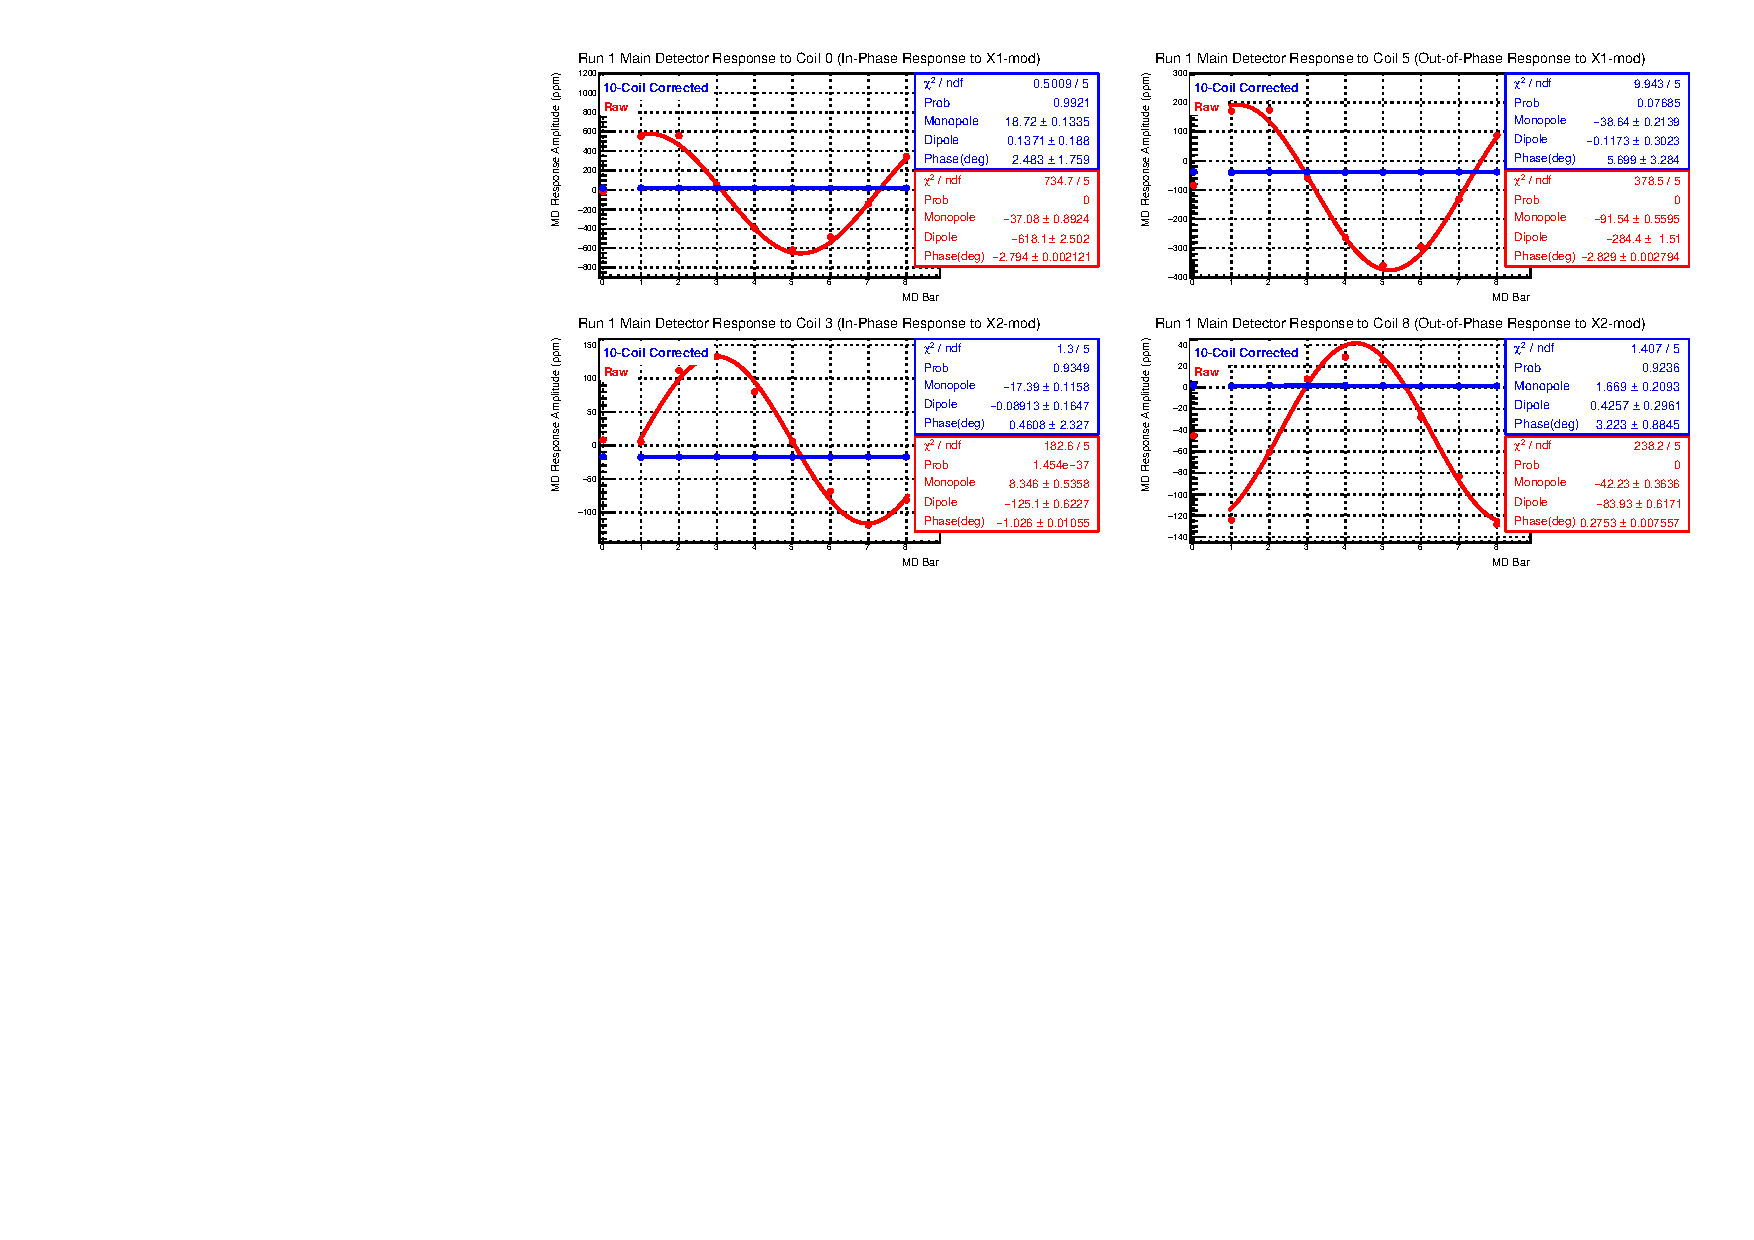
\includegraphics[width=9in]{./Pictures/Run1_X_dipole10-Coil.pdf}
\caption{\label{fig:Run1_10coil_Xdipoles}Responses of individual main detector bars averaged over Run 1 to X-type modulation coils before correction and after correction using a full 10-Coil analysis. The dipole response is given by the amplitude of the sinusoid while the monopole is the offset.}
\end{center}
\end{figure}
\begin{figure}[!ht]
\begin{center}
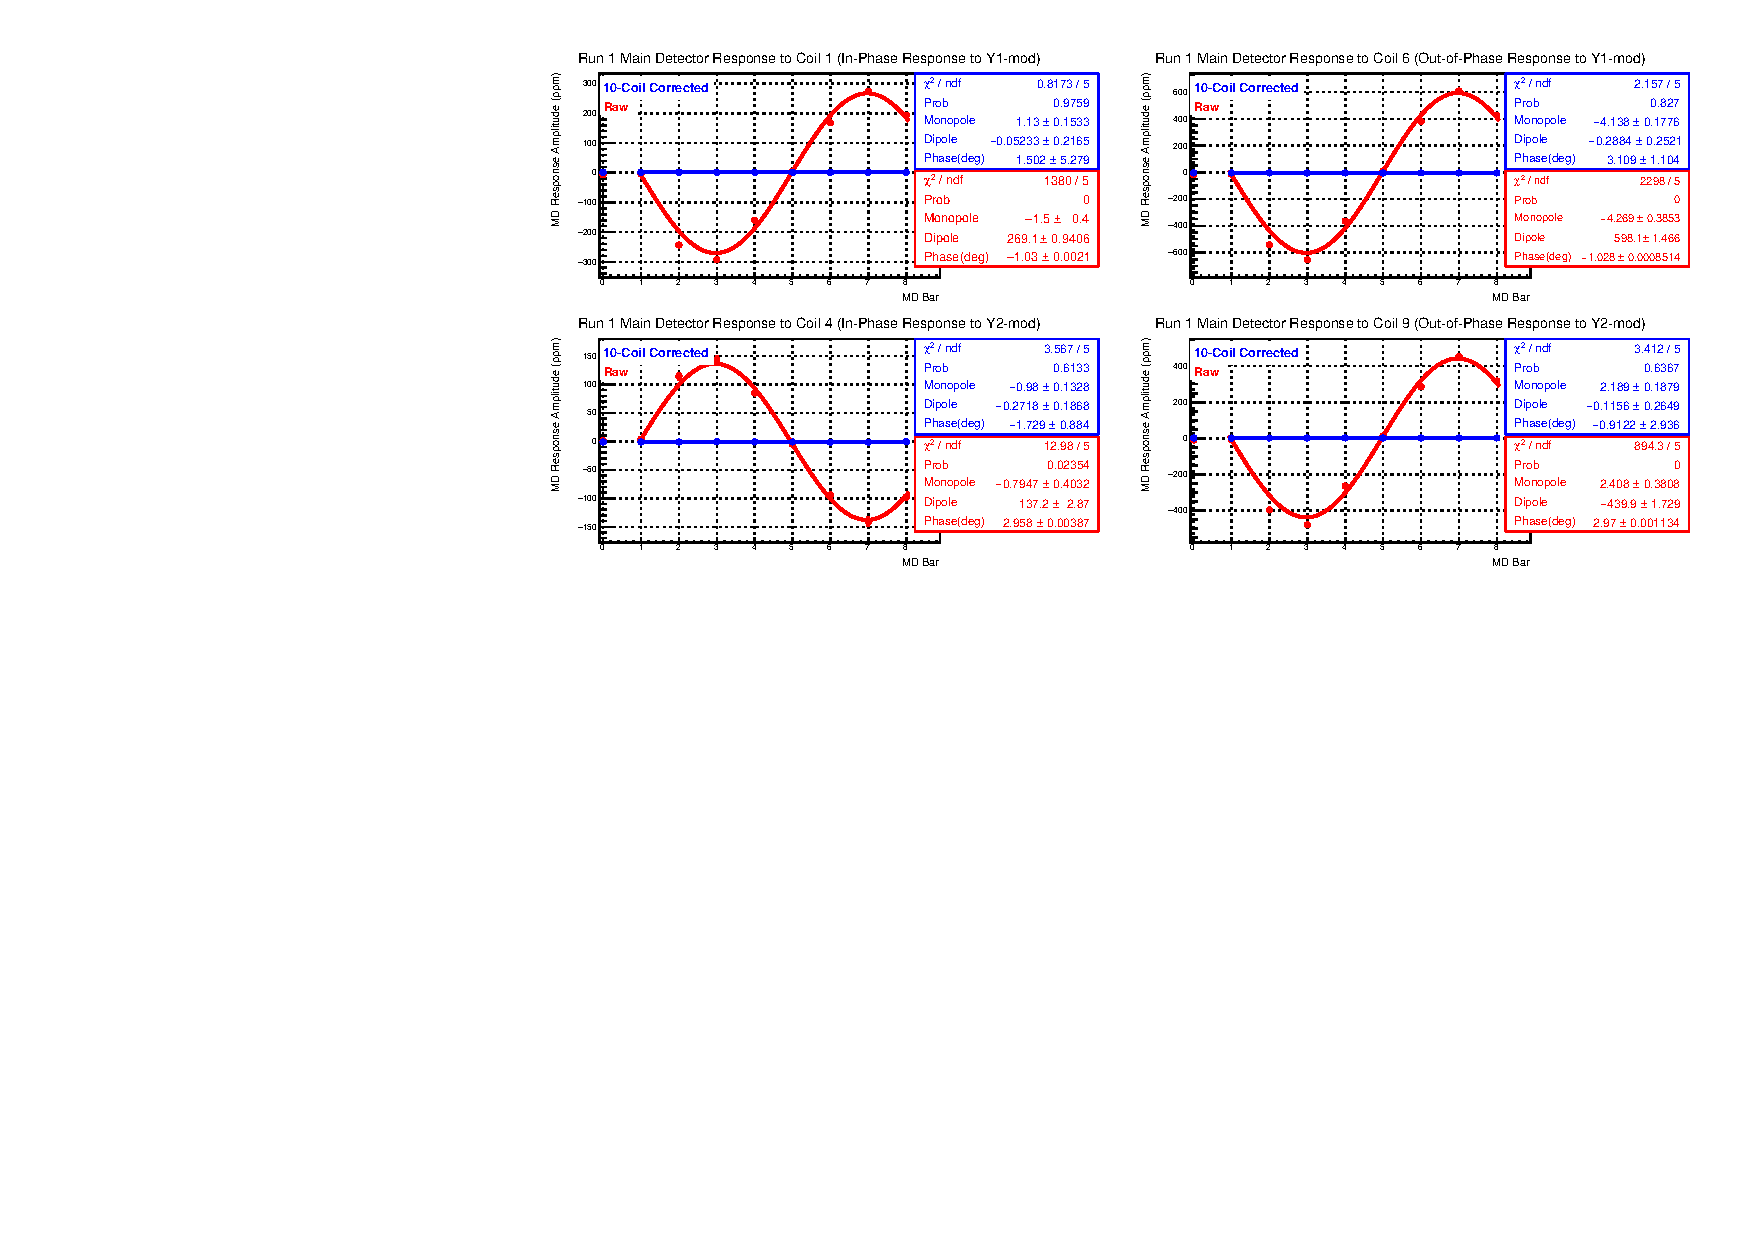
\includegraphics[width=9in]{./Pictures/Run1_Y_dipole10-Coil.pdf}
\caption{\label{fig:Run1_10coil_Ydipoles}Responses of individual main detector bars averaged over Run 1 to Y-type modulation coils before correction and after correction using a full 10-Coil analysis. The dipole response is given by the amplitude of the sinusoid while the monopole is the offset.}
\end{center}
\end{figure}

\begin{figure}[!ht]
\begin{center}
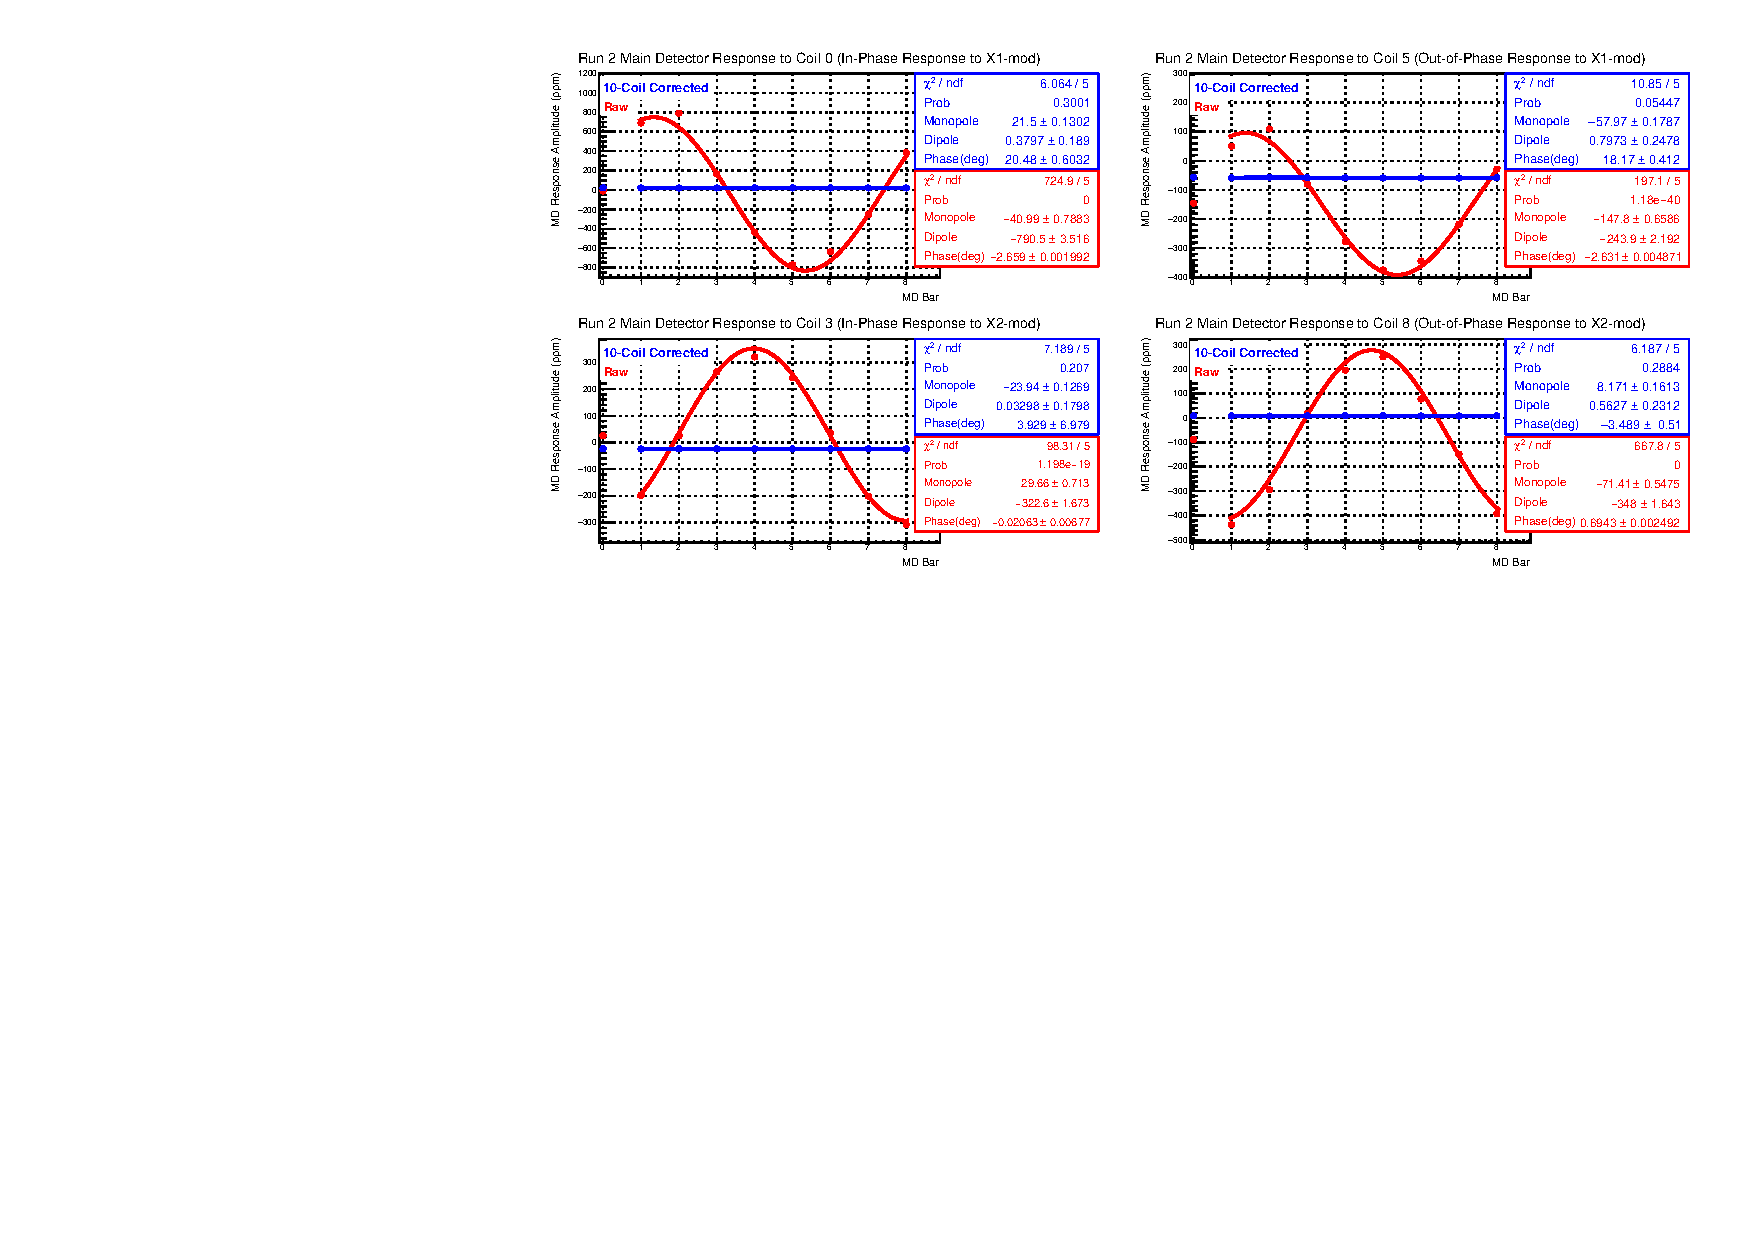
\includegraphics[width=9in]{./Pictures/Run2_X_dipole10-Coil.pdf}
\caption{\label{fig:Run2_10coil_Xdipoles_app}Responses of individual main detector bars averaged over Run 2 to X-type modulation coils before correction and after correction using a full 10-Coil analysis. The dipole response is given by the amplitude of the sinusoid while the monopole is the offset.}
\end{center}
\end{figure}

\begin{figure}[!ht]
\begin{center}
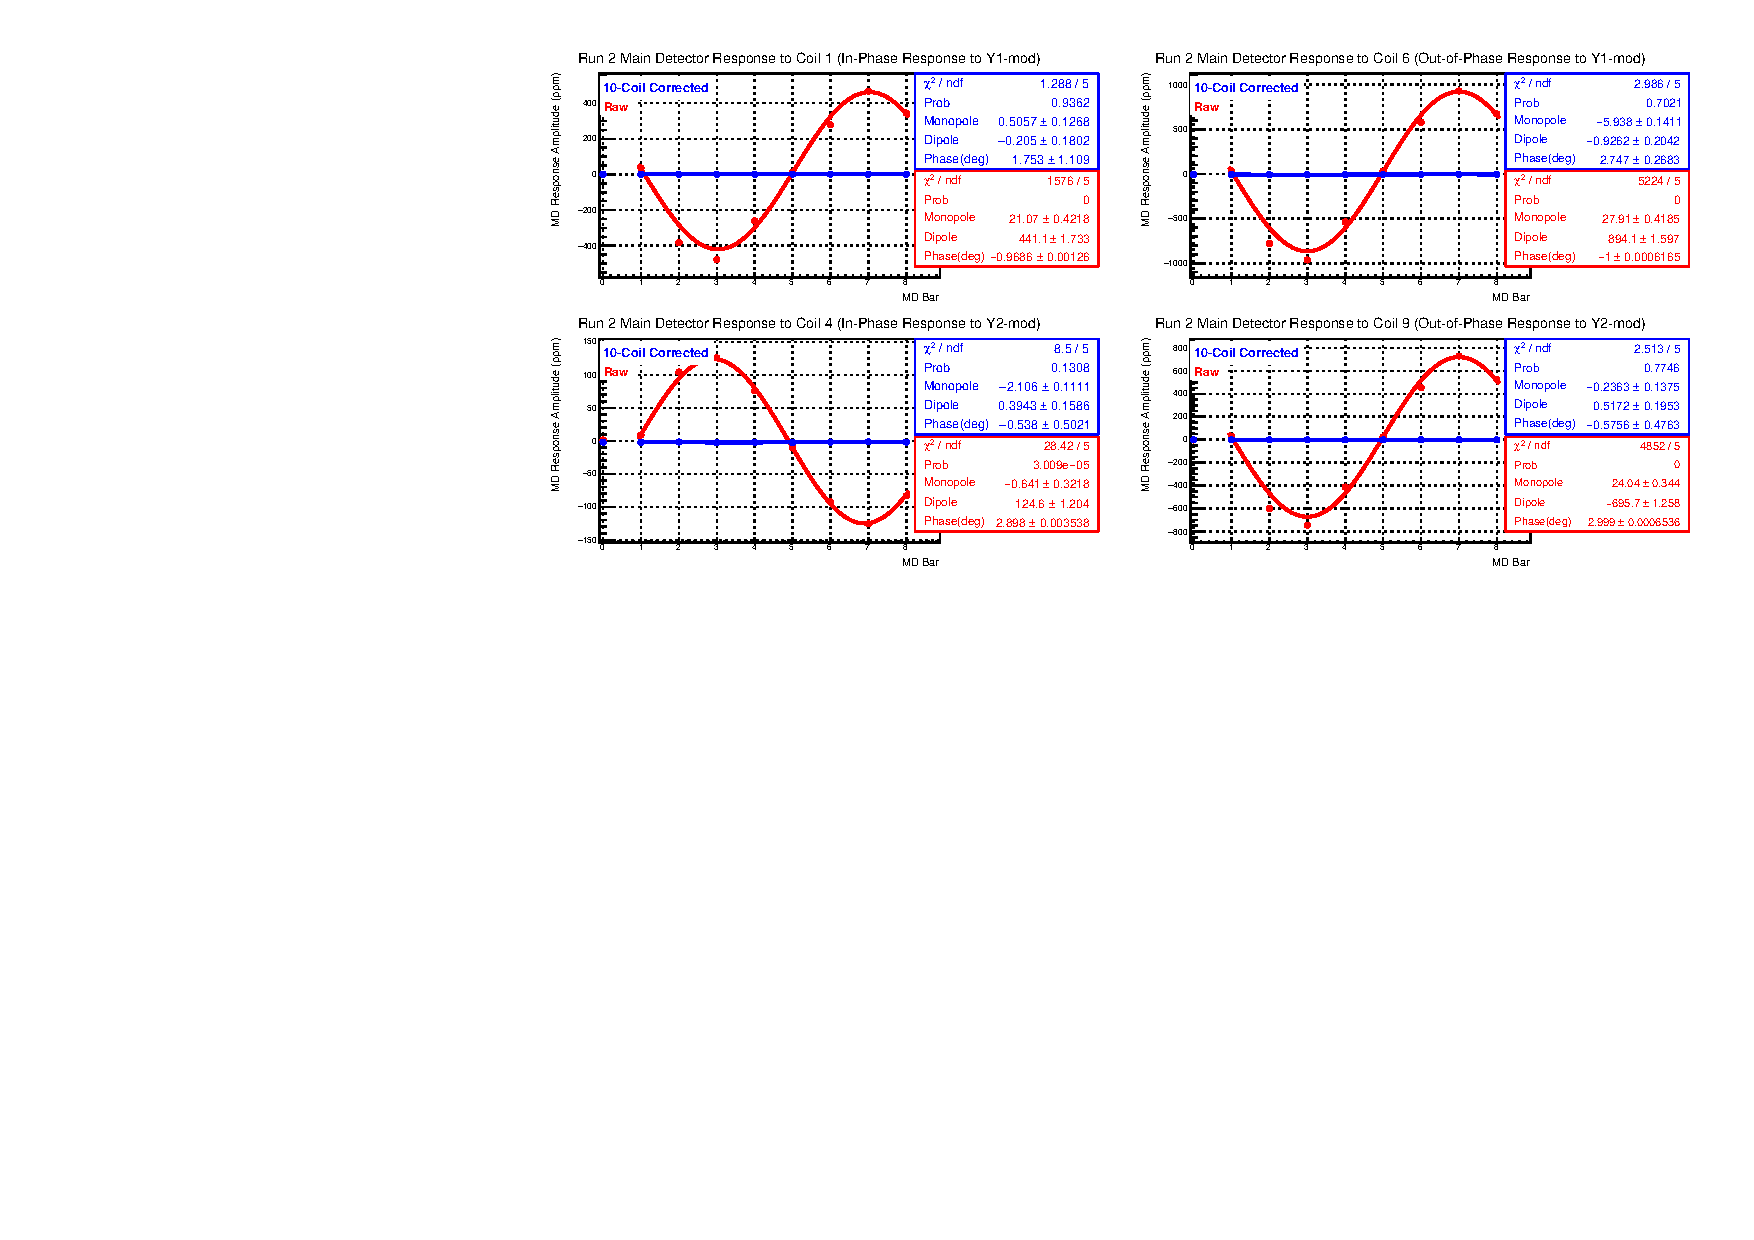
\includegraphics[width=9in]{./Pictures/Run2_Y_dipole10-Coil.pdf}
\caption{\label{fig:Run2_10coil_Ydipoles_app}Responses of individual main detector bars averaged over Run 2 to Y-type modulation coils before correction and after correction using a full 10-Coil analysis. The dipole response is given by the amplitude of the sinusoid while the monopole is the offset.}
\end{center}
\end{figure}

\begin{figure}[!ht]
\begin{center}
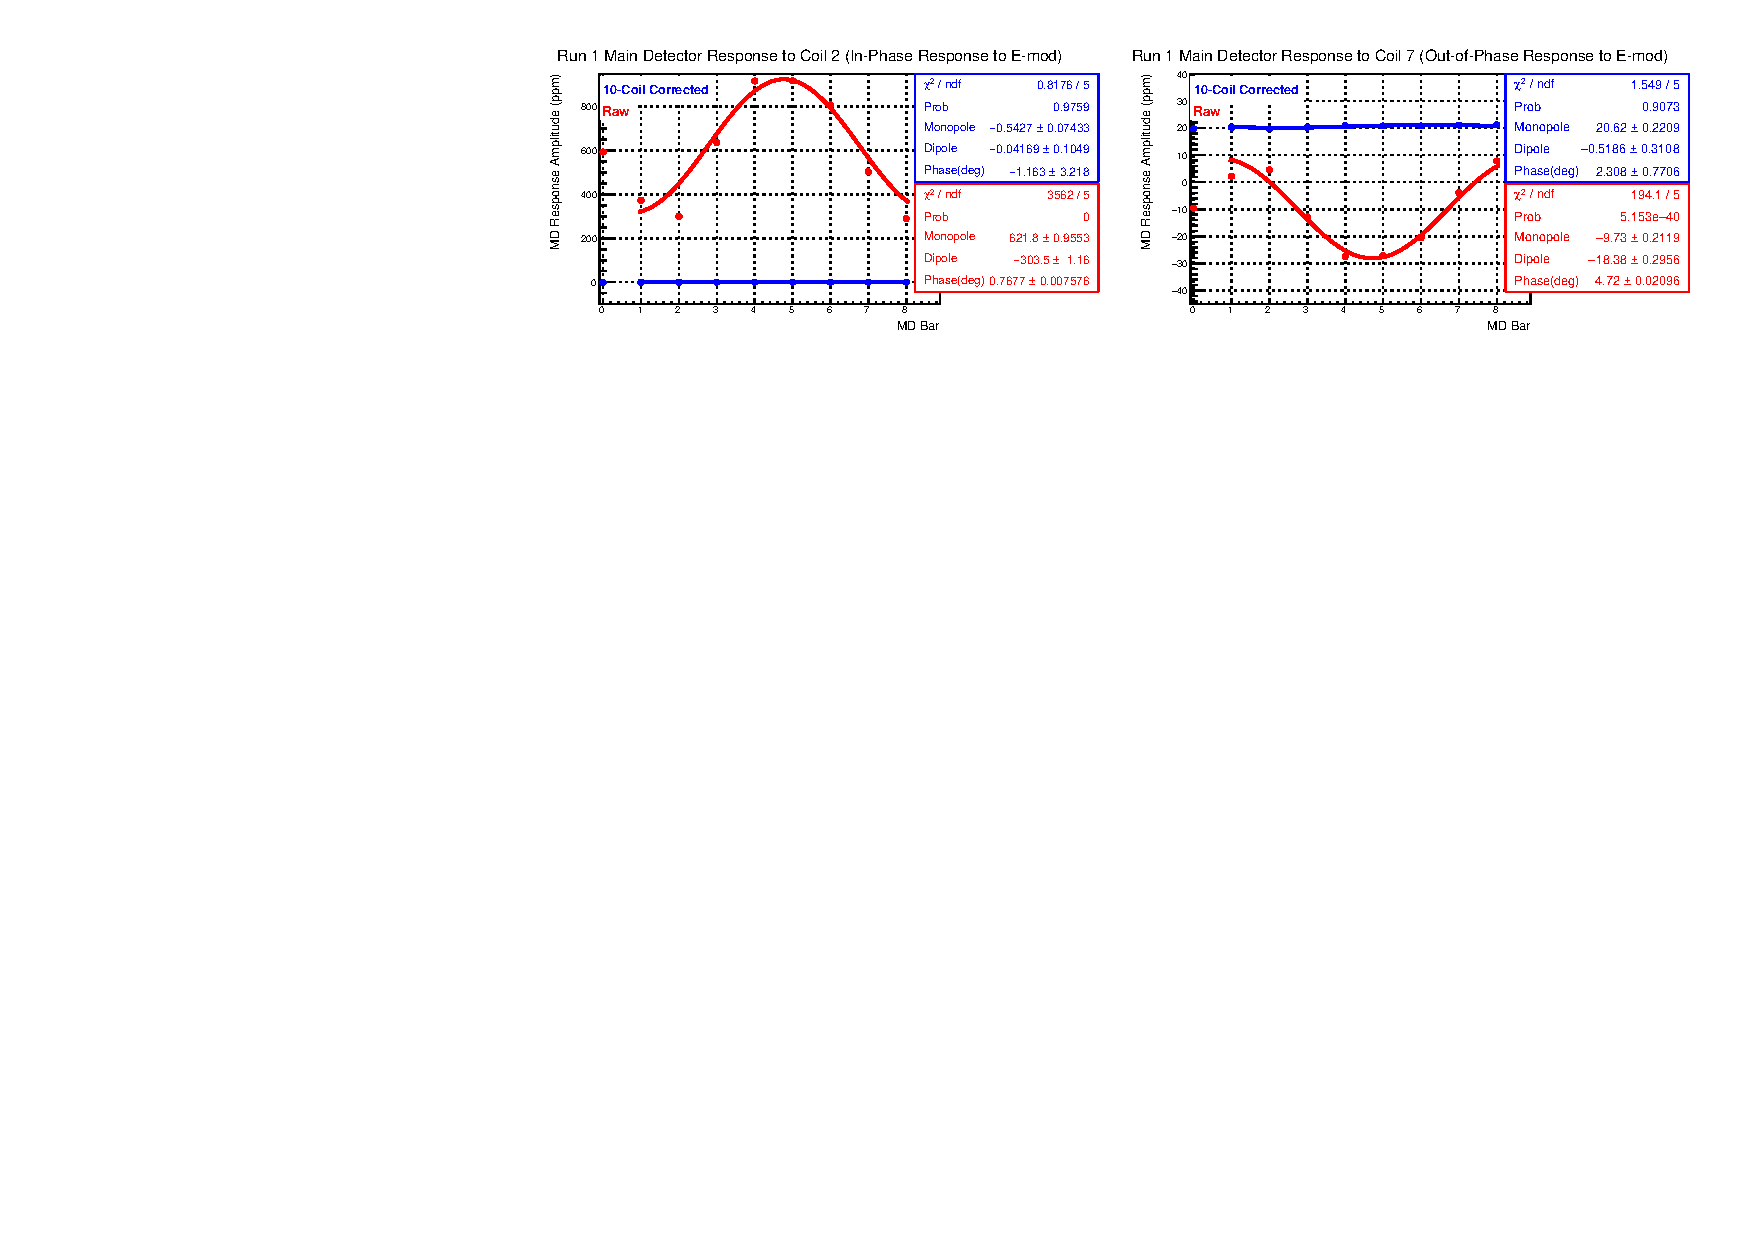
\includegraphics[width=9in]{./Pictures/Run1_E_dipole10-Coil.pdf}
\caption{\label{fig:Run1_10coil_Edipoles_app}Responses of individual main detector bars averaged over Run 1 to energy modulation coils before correction and after correction using a full 10-Coil analysis. The dipole response is given by the amplitude of the sinusoid while the monopole is the offset.}
\end{center}
\end{figure}

\begin{figure}[!ht]
\begin{center}
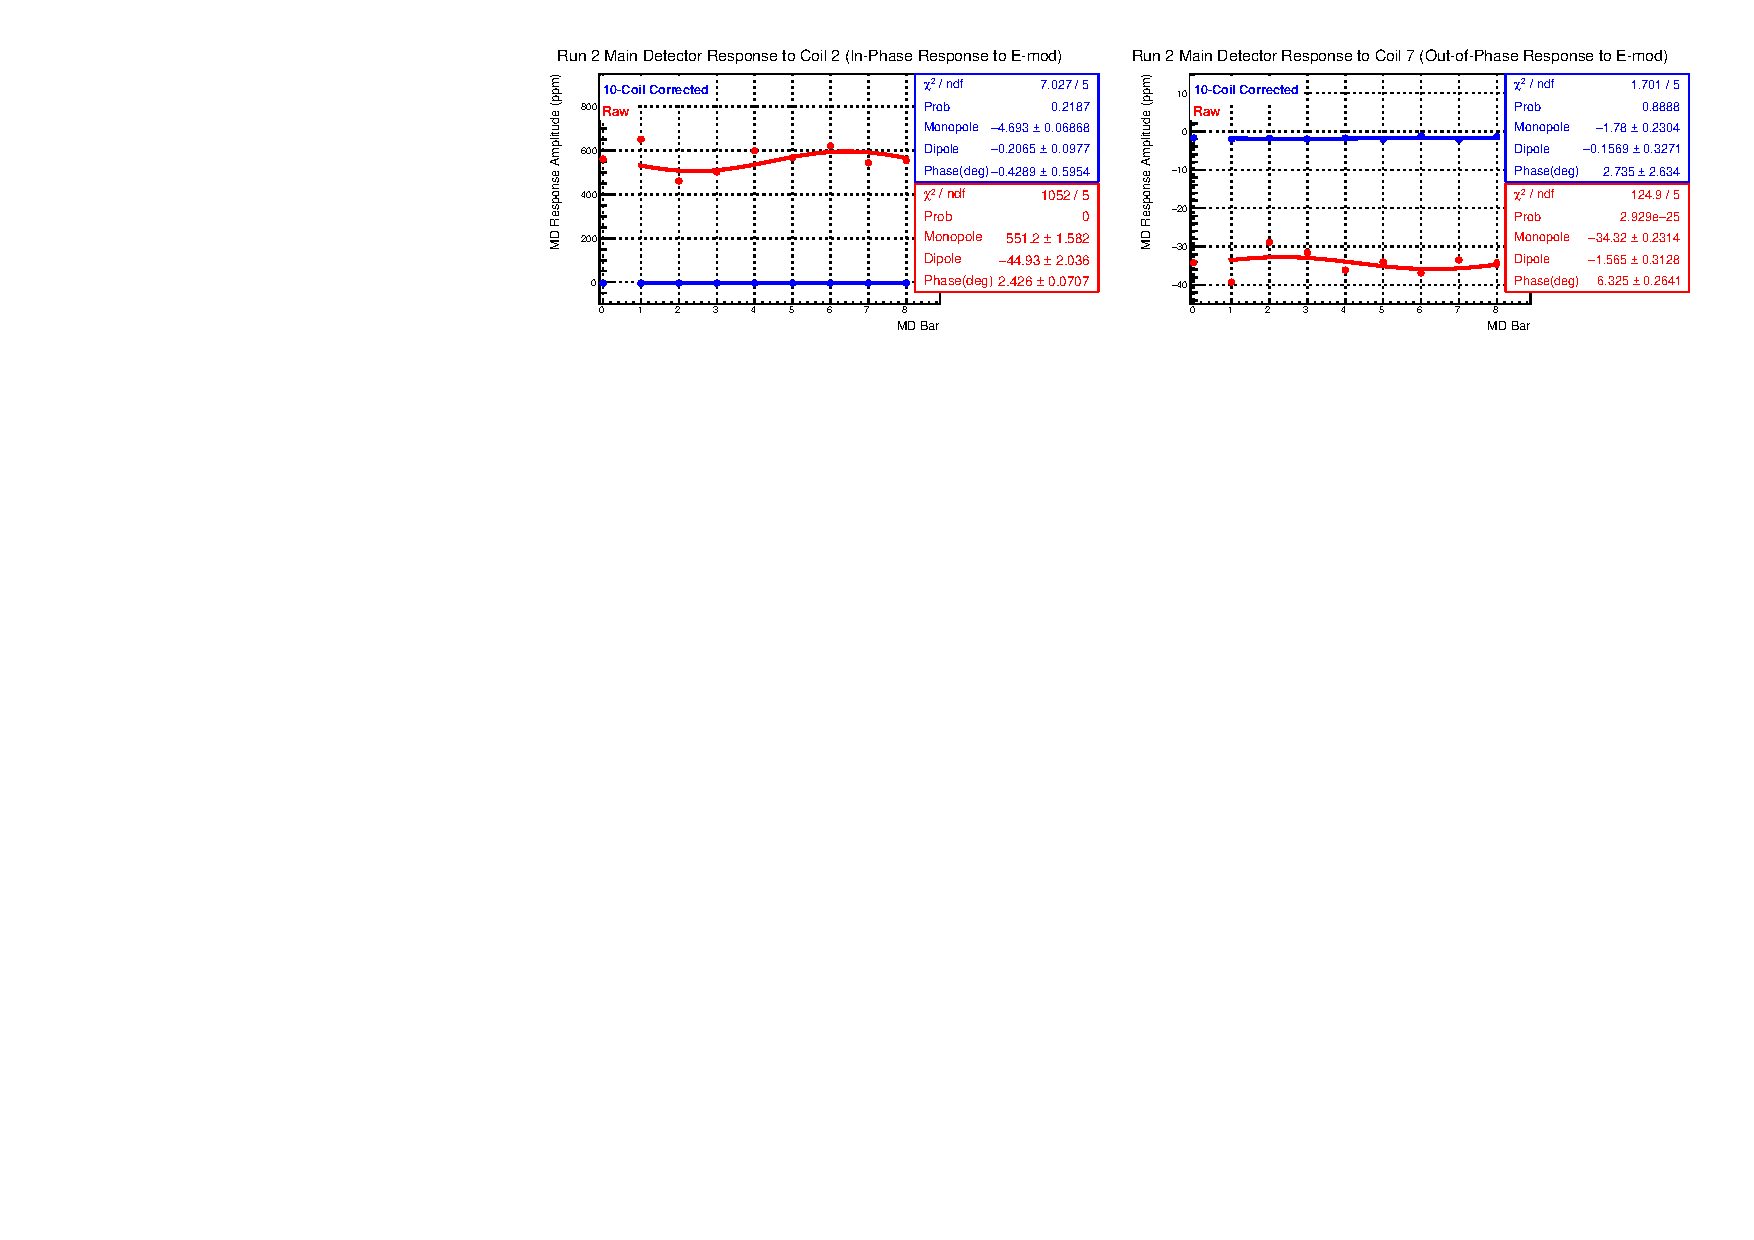
\includegraphics[width=9in]{./Pictures/Run2_E_dipole10-Coil.pdf}
\caption{\label{fig:Run2_10coil_Edipoles_app}Responses of individual main detector bars averaged over Run 2 to energy modulation coils before correction and after correction using a full 10-Coil analysis. The dipole response is given by the amplitude of the sinusoid while the monopole is the offset.}
\end{center}
\end{figure}

\begin{figure}[!ht]
\begin{center}
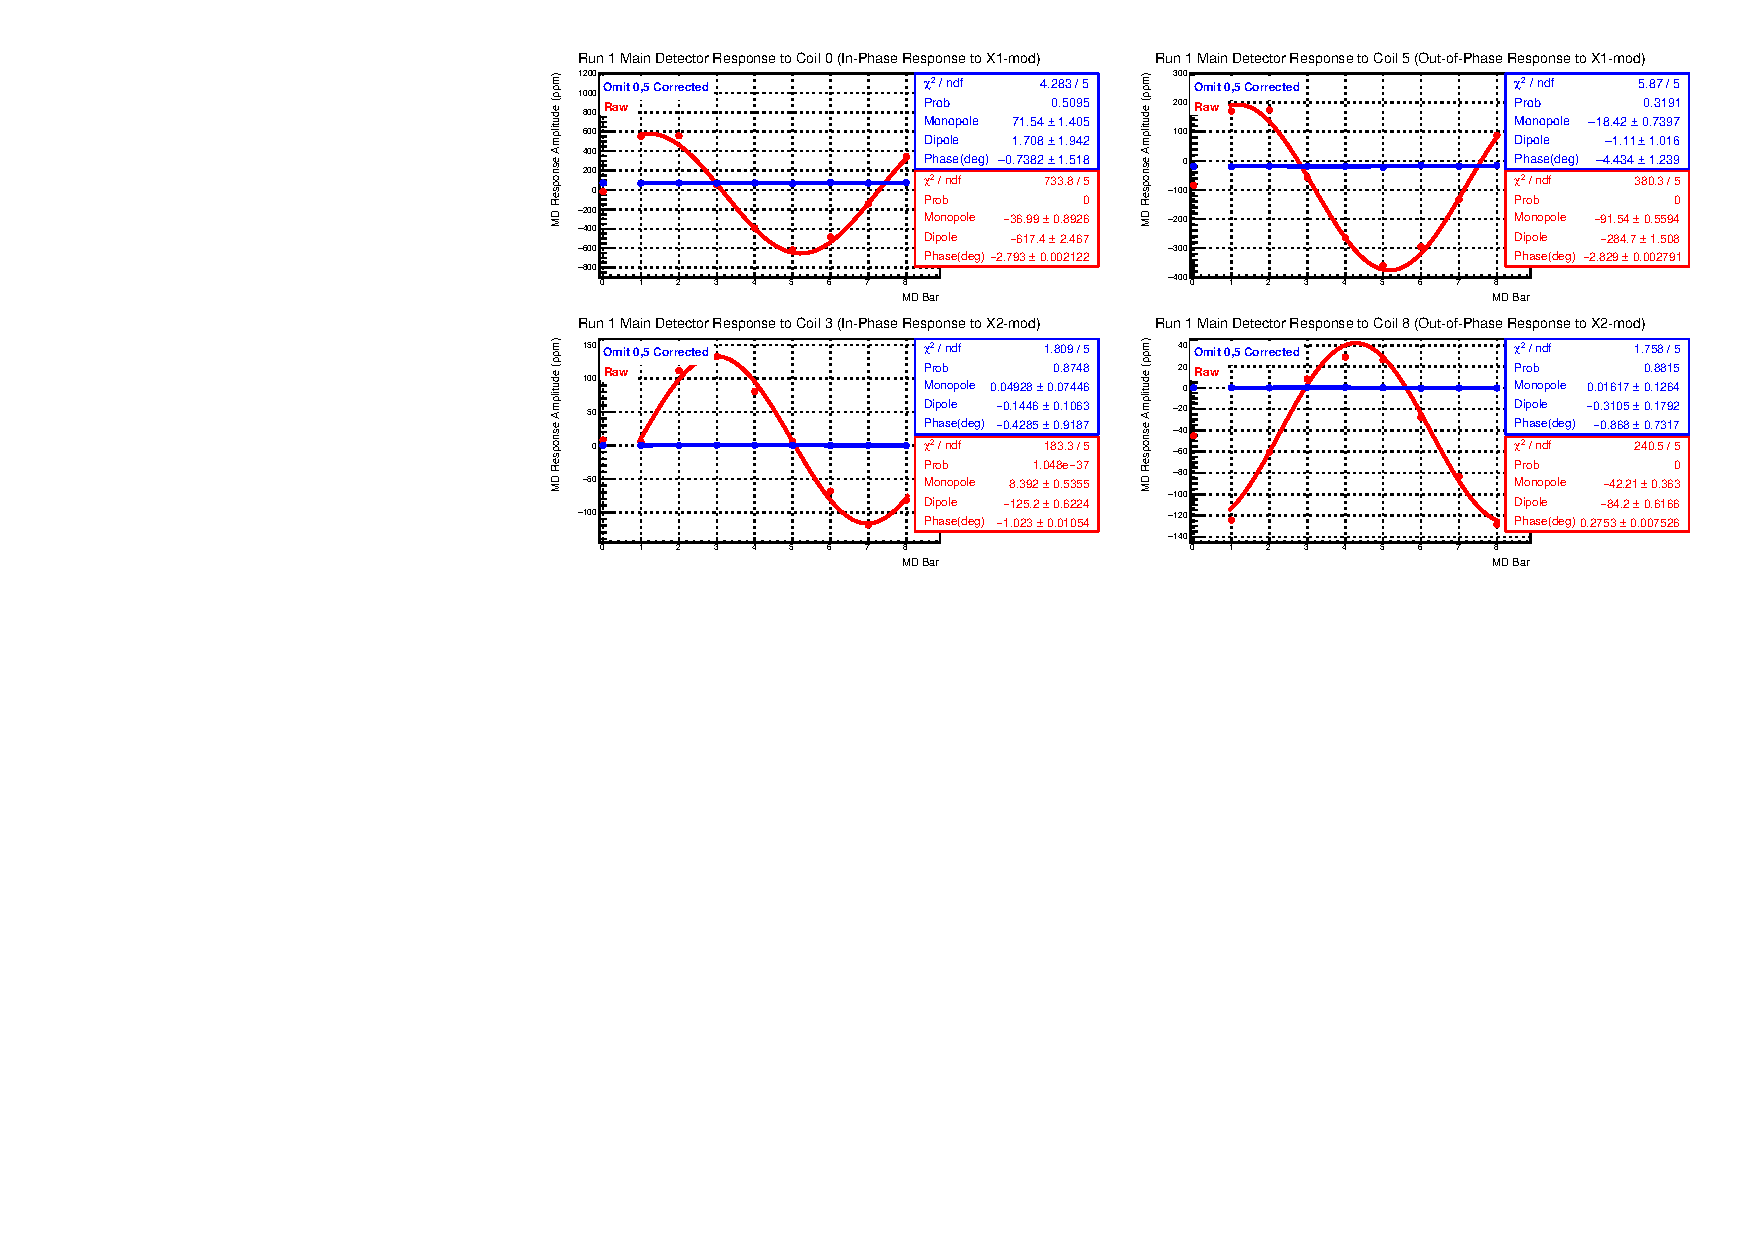
\includegraphics[width=9in]{./Pictures/Run1_X_dipoleOmit05.pdf}
\caption{\label{fig:Run1_Omit05_Xdipoles}Responses of individual main detector bars averaged over Run 1 to X-type modulation coils before correction and after correction using the ``Omit 0,5'' analysis. The dipole response is given by the amplitude of the sinusoid while the monopole is the offset.}
\end{center}
\end{figure}
\begin{figure}[!ht]
\begin{center}
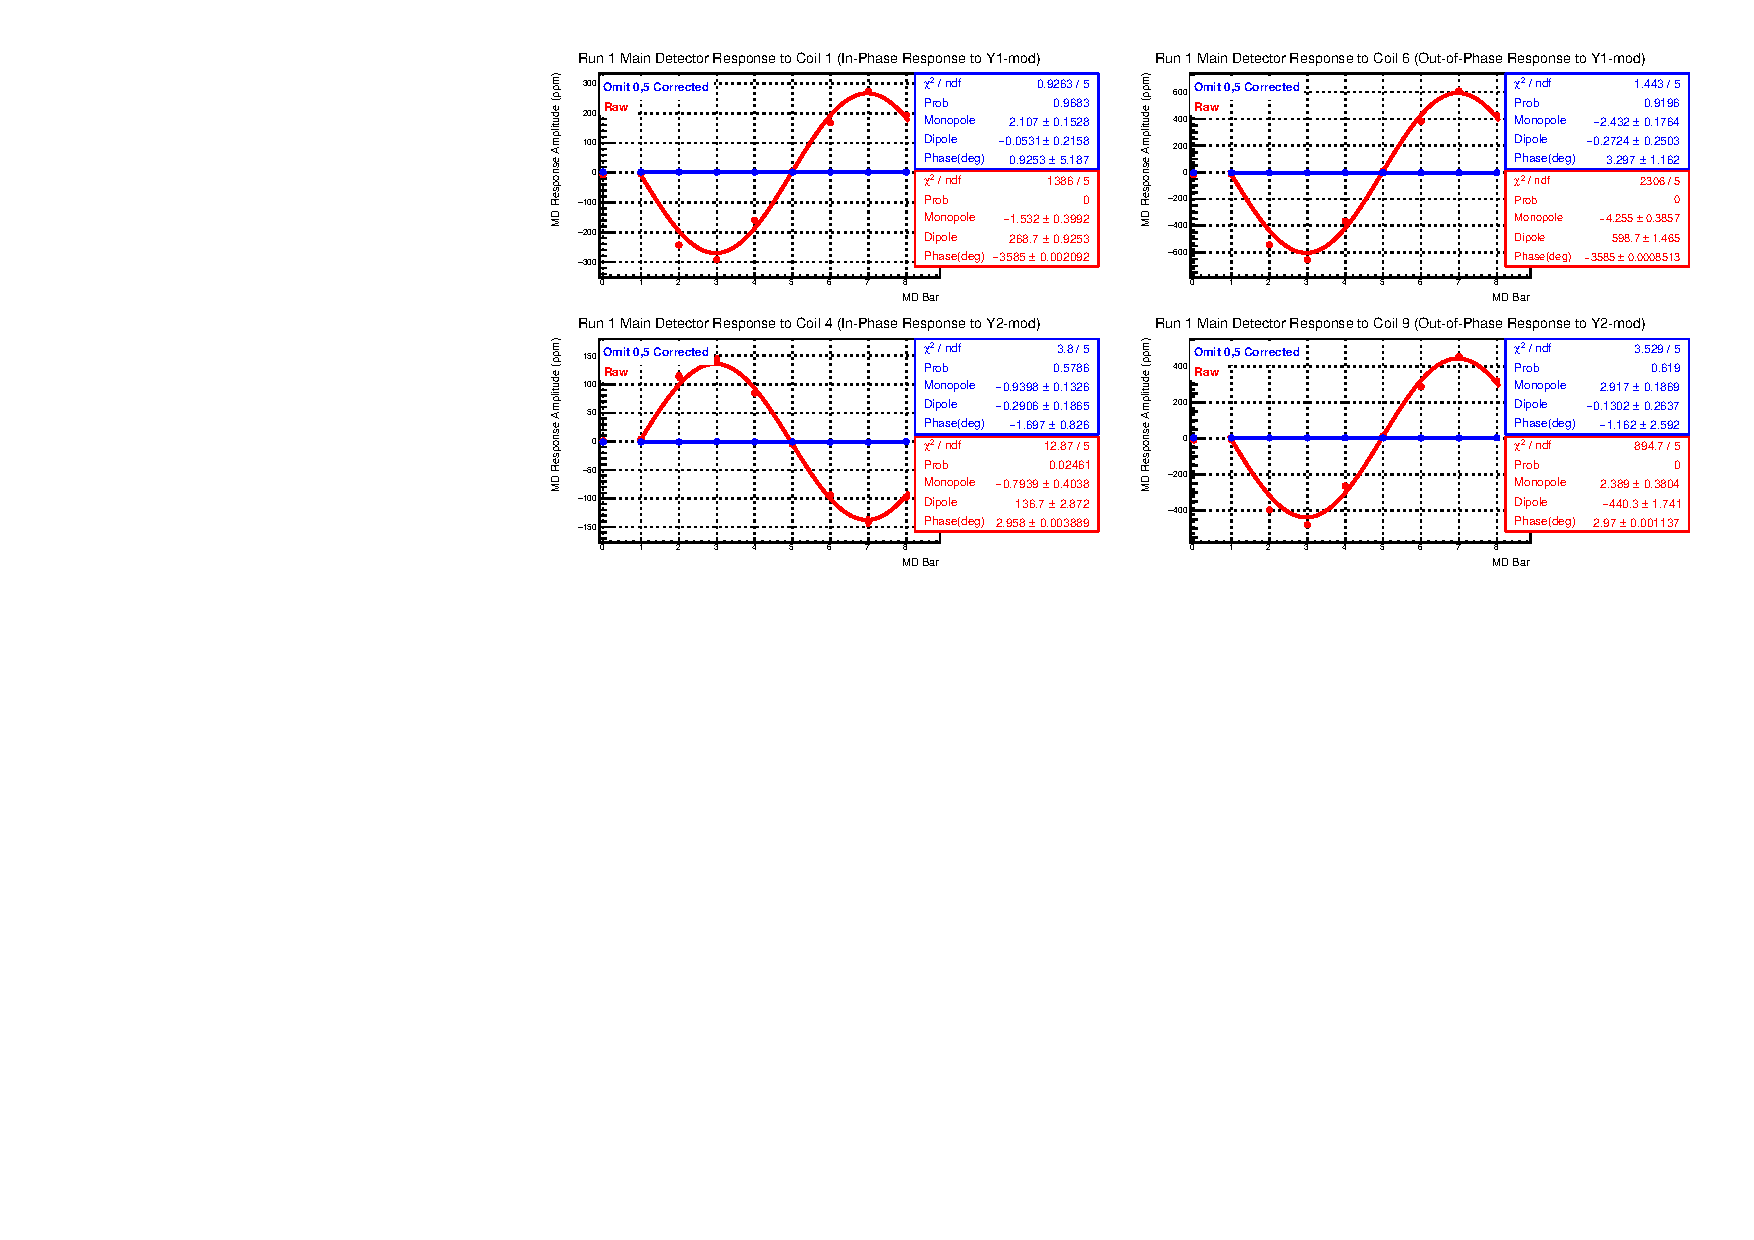
\includegraphics[width=9in]{./Pictures/Run1_Y_dipoleOmit05.pdf}
\caption{\label{fig:Run1_Omit05_Ydipoles}Responses of individual main detector bars averaged over Run 1 to Y-type modulation coils before correction and after correction using the ``Omit 0,5'' analysis. The dipole response is given by the amplitude of the sinusoid while the monopole is the offset.}
\end{center}
\end{figure}

\begin{figure}[!ht]
\begin{center}
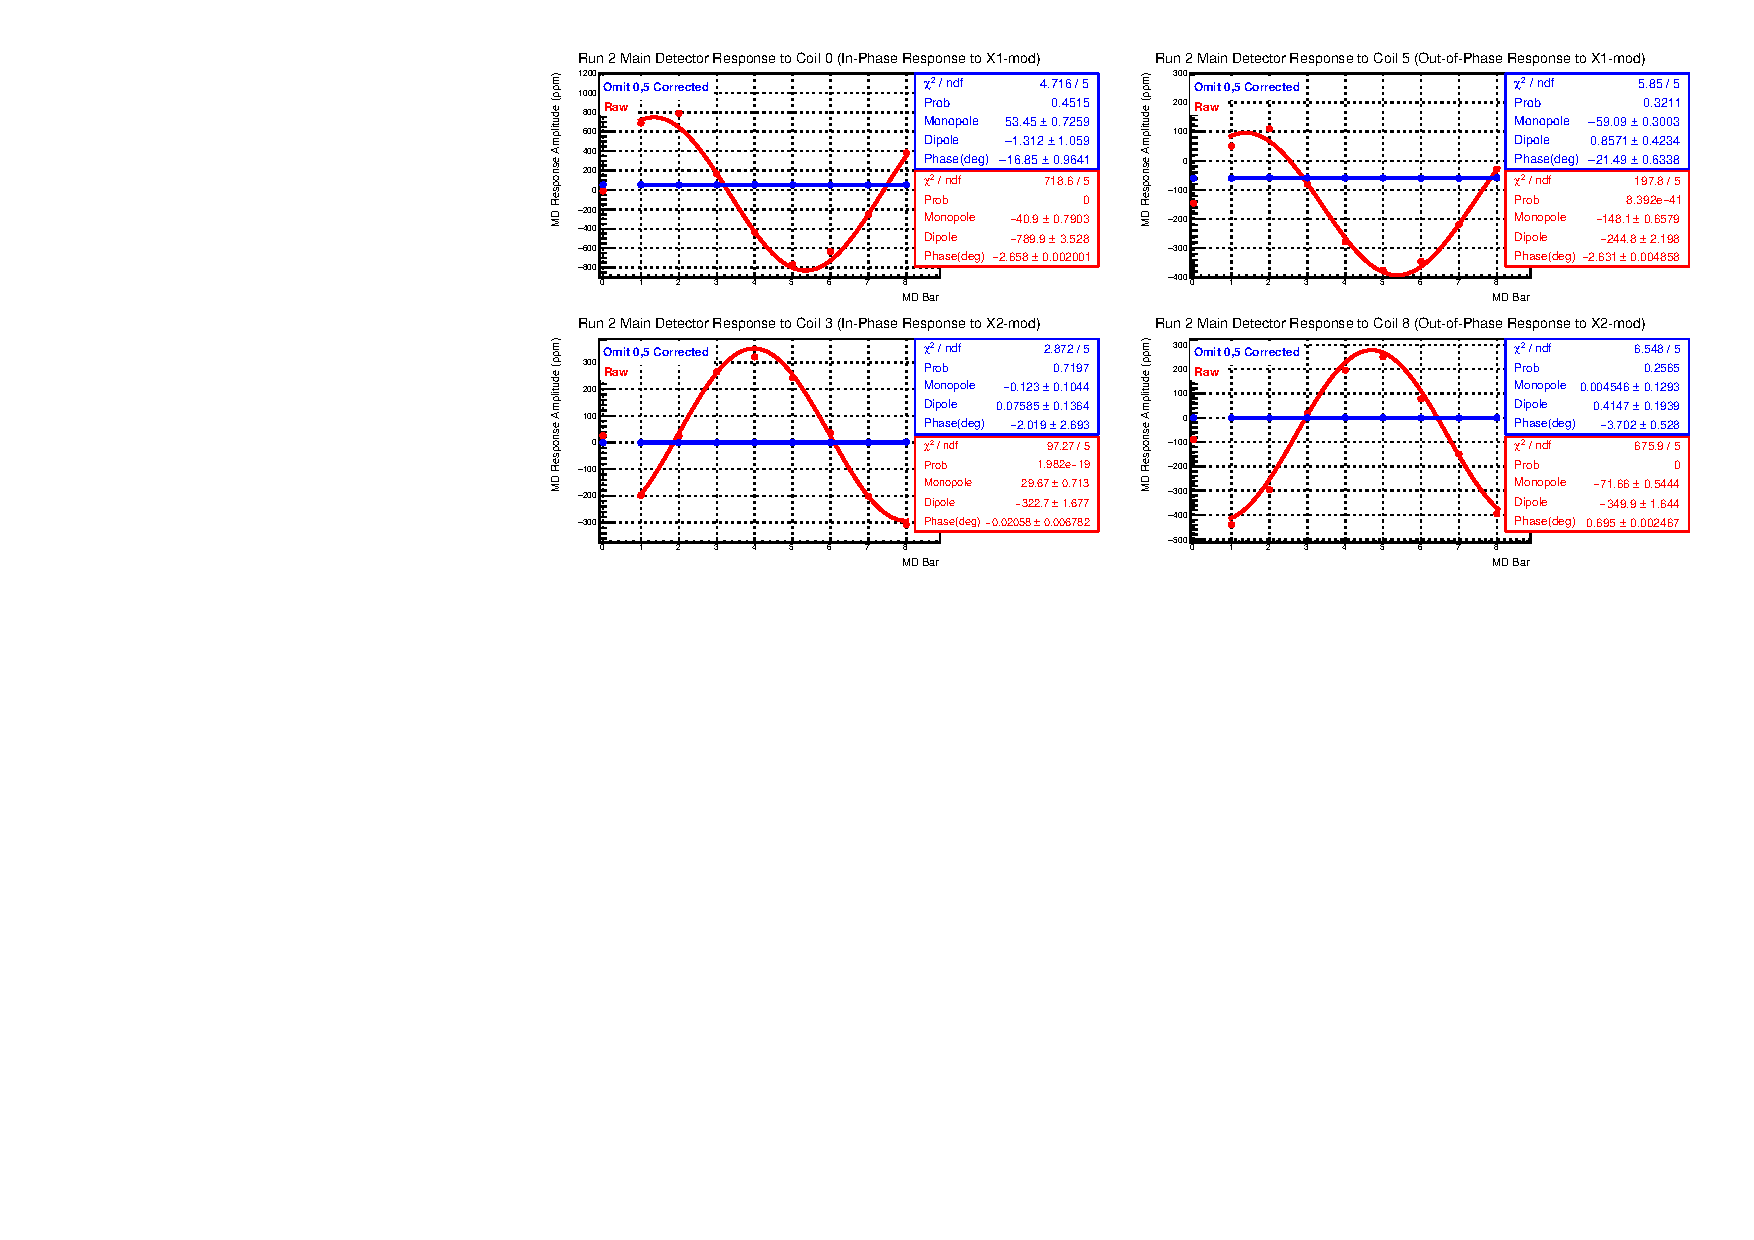
\includegraphics[width=9in]{./Pictures/Run2_X_dipoleOmit05.pdf}
\caption{\label{fig:Run2_Omit05_Xdipoles_app}Responses of individual main detector bars averaged over Run 2 to X-type modulation coils before correction and after correction using the ``Omit 0,5'' analysis. The dipole response is given by the amplitude of the sinusoid while the monopole is the offset.}
\end{center}
\end{figure}

\begin{figure}[!ht]
\begin{center}
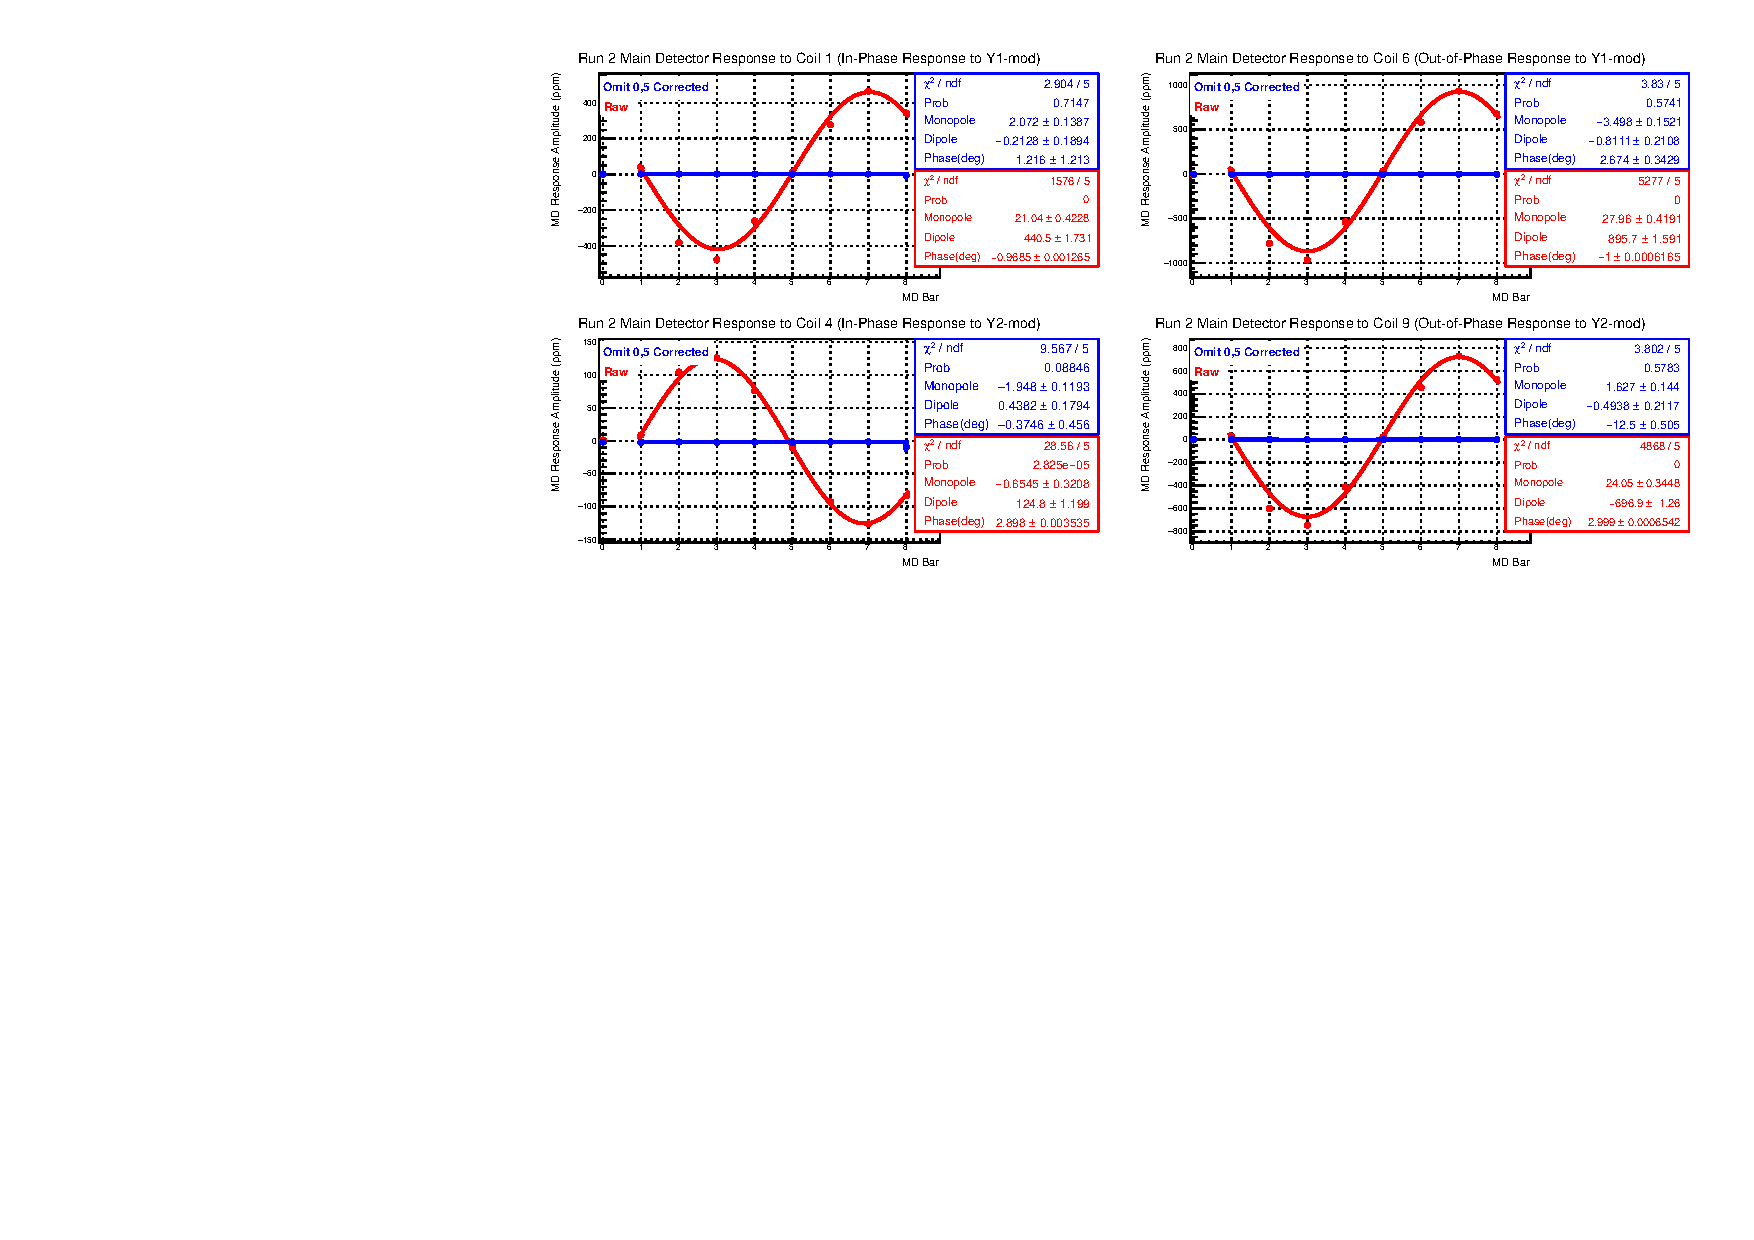
\includegraphics[width=9in]{./Pictures/Run2_Y_dipoleOmit05.pdf}
\caption{\label{fig:Run2_Omit05_Ydipoles_app}Responses of individual main detector bars averaged over Run 2 to Y-type modulation coils before correction and after correction using the ``Omit 0,5'' analysis. The dipole response is given by the amplitude of the sinusoid while the monopole is the offset.}
\end{center}
\end{figure}

\begin{figure}[!ht]
\begin{center}
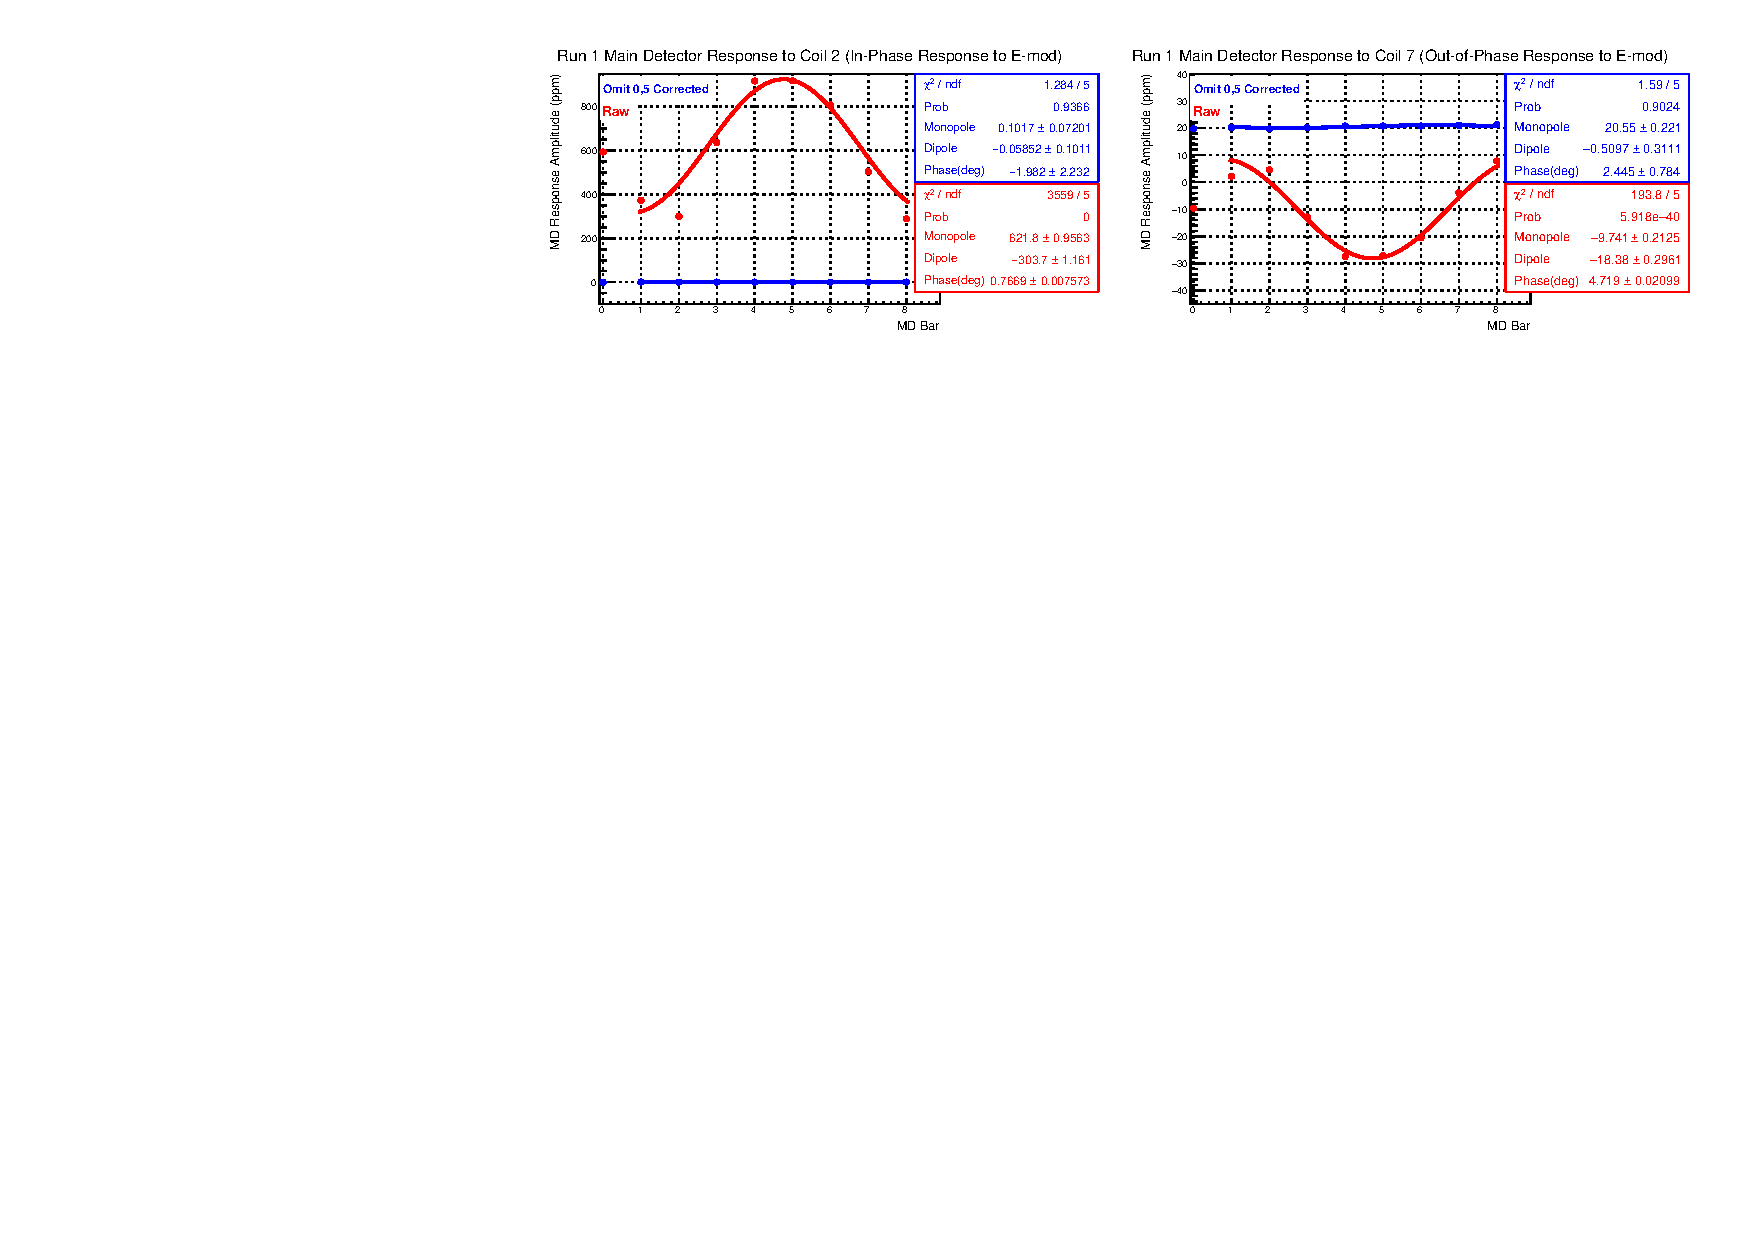
\includegraphics[width=9in]{./Pictures/Run1_E_dipoleOmit05.pdf}
\caption{\label{fig:Run1_Omit05_Ydipoles_app}Responses of individual main detector bars averaged over Run 1 to energy modulation coils before correction and after correction using the ``Omit 0,5'' analysis. The dipole response is given by the amplitude of the sinusoid while the monopole is the offset.}
\end{center}
\end{figure}

\begin{figure}[!ht]
\begin{center}
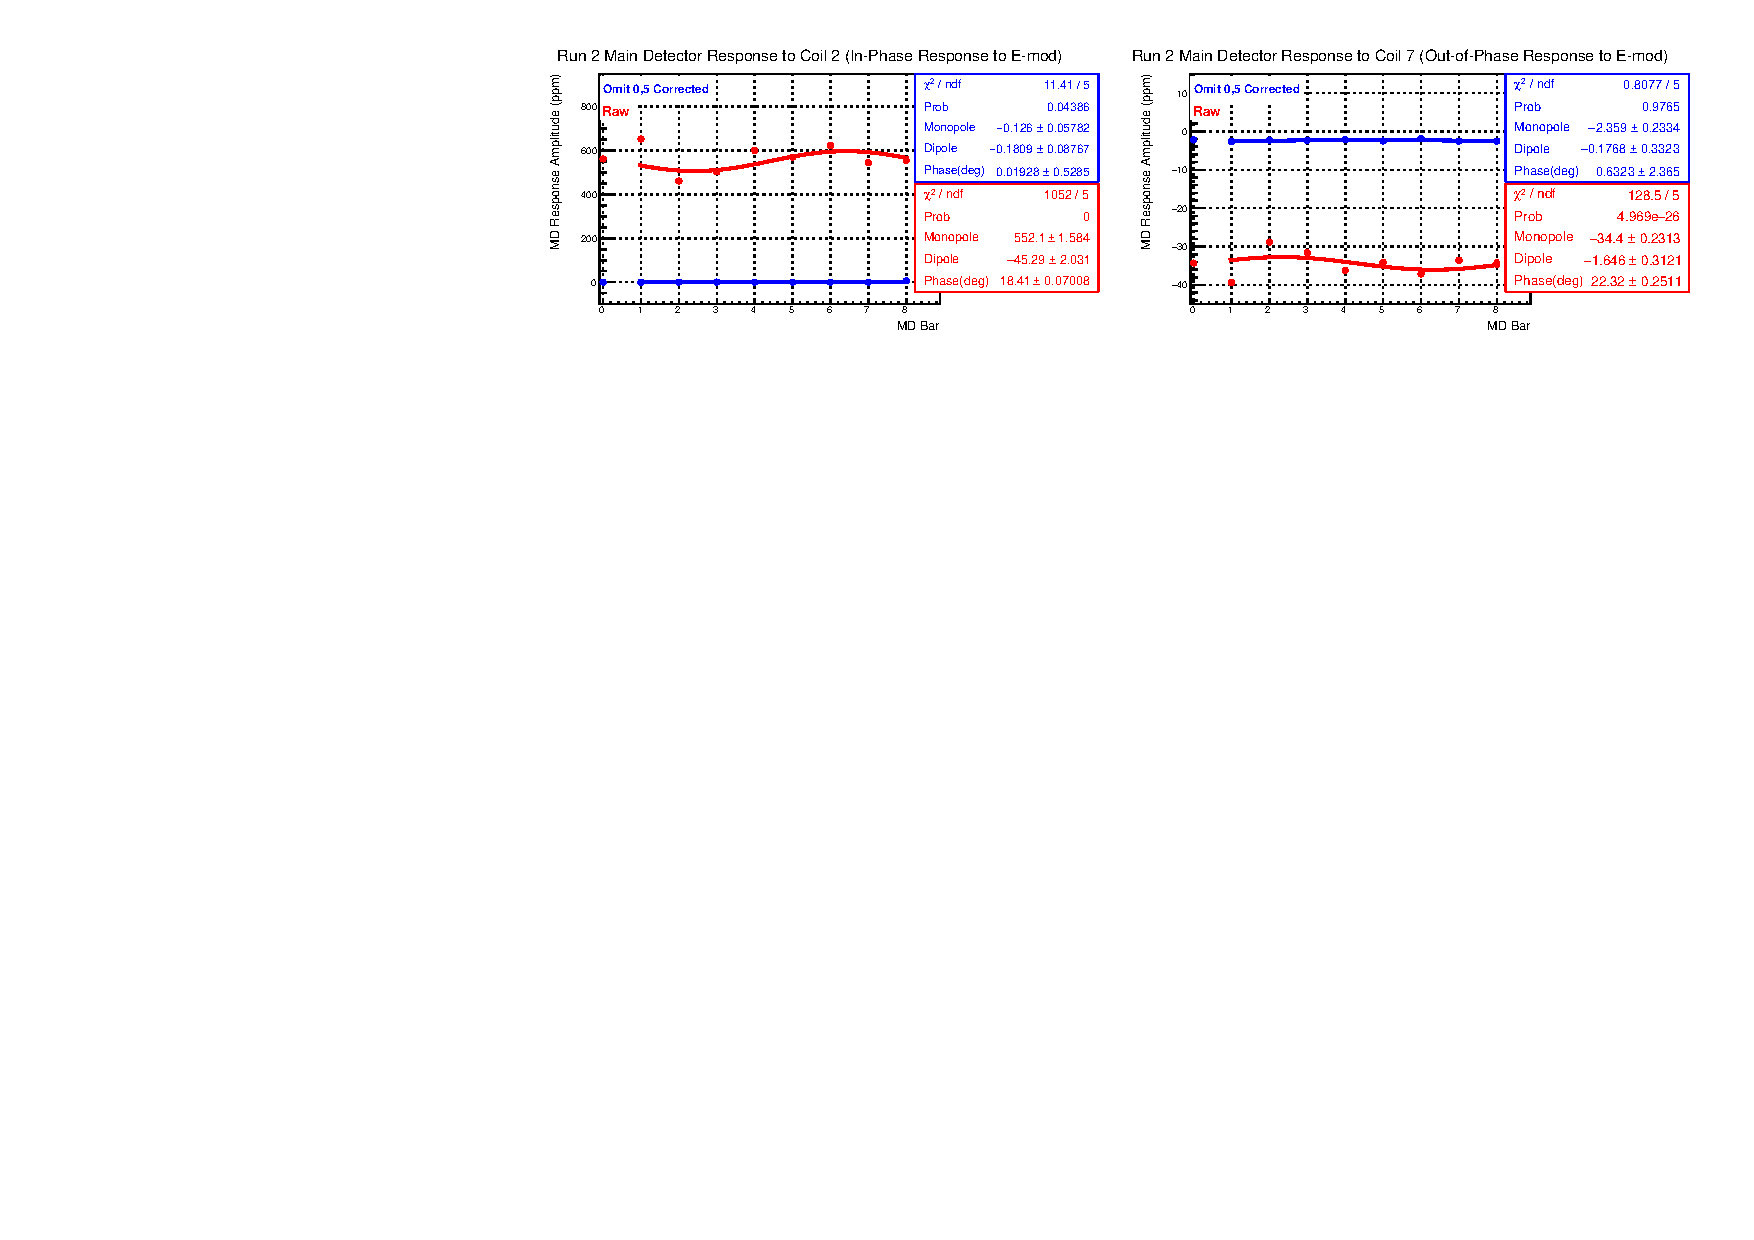
\includegraphics[width=9in]{./Pictures/Run2_E_dipoleOmit05.pdf}
\caption{\label{fig:Run2_Omit05_Edipoles_app}Responses of individual main detector bars averaged over Run 2 to energy modulation coils before correction and after correction using the ``Omit 0,5'' analysis. The dipole response is given by the amplitude of the sinusoid while the monopole is the offset.}
\end{center}
\end{figure}

\begin{figure}[!ht]
\begin{center}
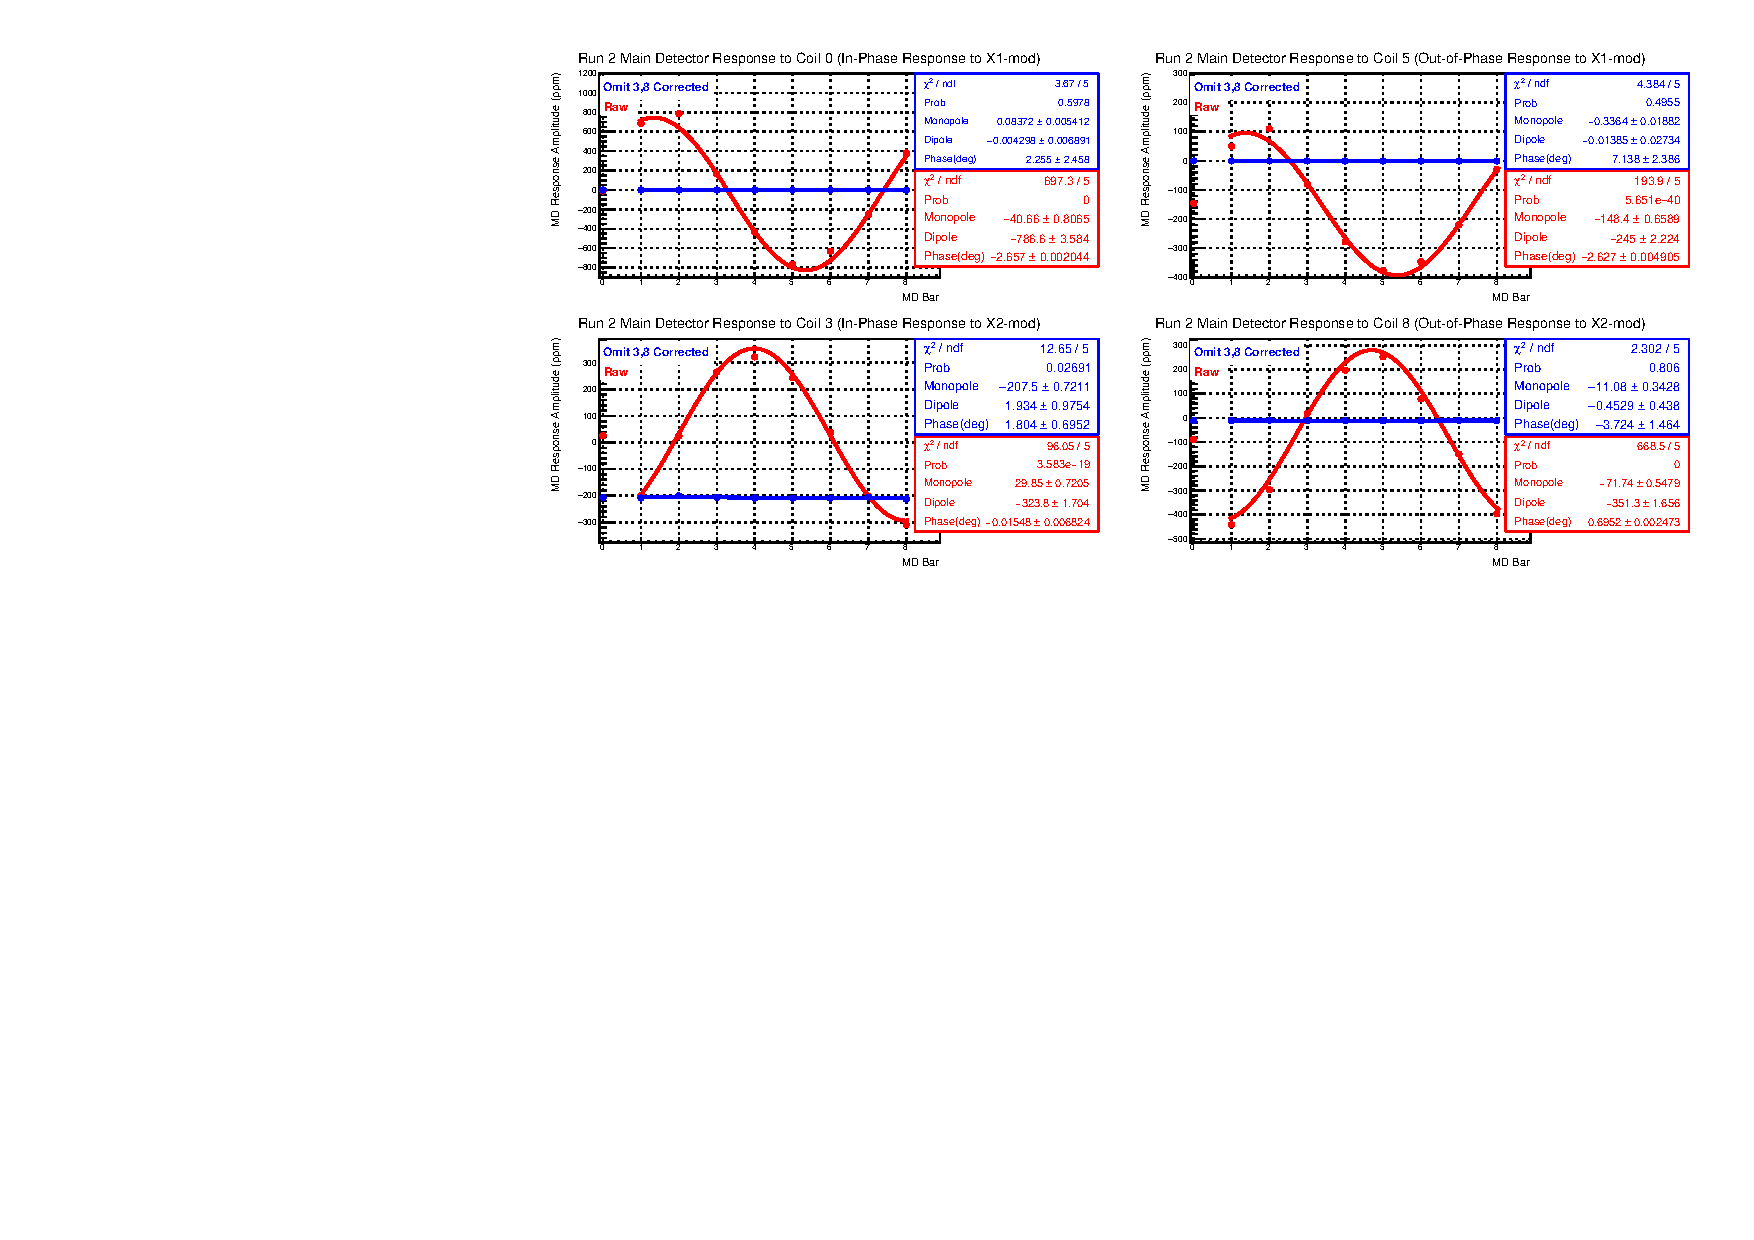
\includegraphics[width=9in]{./Pictures/Run2_X_dipoleOmit3_8.pdf}
\caption{\label{fig:Run2_Omit38_Edipoles}Responses of individual main detector bars averaged over Run 2 to X-type modulation coils before correction and after correction using the ``Omit 3,8'' analysis considered unreliable due to large residual correlations it produces between the main detector and the monitors (see table \ref{tab:run2_residual_correlations_table}). Notice the large monopole residual in the dipole response is given by the amplitude of the sinusoid while the monopole is the offset.}
\end{center}
\end{figure}
\end{landscape}
